\section*{Bases de datos distribuidas (DDB)}
Se definen como colecciones de BDs \textbf{lógicamente relacionadas} y \textbf{distribuidas} a través de una red de computadoras. Son manejadas por un \textbf{DDBMS} que busca hacer transparente la distribución al usuario y que sus nodos cumplan con una serie de características. \\
Dada una consulta su estrategia de ejecución depende del \textbf{tipo y la topología de la interconexión} entre los nodos de la red (LAN, WAN, conexión directa, conectividad). También depende de la \textbf{forma} en que esté distribuida la información (dada una junta debemos atender a la cantidad de datos que deben ser transeridos).



\subsection*{Fragmentación}
Los \textbf{fragmentos} son las partes resultantes de dividir la DB en unidades lógicas. La fragmentación puede ser:
\begin{itemize}
    \item \textbf{Horizontal (sharding):} Subdivisión en \textbf{subconjuntos de tuplas} de la relación original. Es análoga al operador \texttt{SELECT} y de comprender a todas las tuplas se denomina \textbf{completa} (puede ser disjunta). Su reconstrucción viene dada por \texttt{UNION}. Aumenta el performance de las escrituras y lecturas distribuyendo la carga en distintos nodos, pero reduce el performance de operaciones analíticas al requerir \texttt{UNIONS} cuando se quiere todos los datos de la tabla (ver \hyperlink{olap}{OLAP} y \hyperlink{oltp}{OLTP}).
    \item \textbf{Vertical:} Subdivisión en subrelaciones dadas por un \textbf{subconjunto de columnas} de la original. Es análoga al \textbf{proyector} y si cada atributo está en al menos una proyección y todas comparten sólo la PK se denomina \textbf{completa}. La reconstrucción viene dada por \texttt{OUTER JOIN}. Aumenta el performance de las lecturas y escrituras ya que distribuye la carga en distintos nodos cuando se trata de accesos a pocas columnas, pero a costa que las operaciones que requieran el uso de todas las columnas se vean ralentizadas por la necesidad de realizar \texttt{JOINS}.
    \item \textbf{Mixta:} Combinación de las dos anteriores que puede reconstruir la relación con las operaciones en el orden apropiado.
\end{itemize}
Un \textbf{esquema de fragmentación} de una DB es un conjunto de fragmentos que incluye a todos sus atributos y tuplas, y permite reconstruirla con la secuencia de operaciones apropiada. Por otra parte, un \textbf{esquema de asignación} describe la ubiación de los fragmentos en los nodos de la DDB y de estar uno en más de un lugar se denomina \textbf{replicado}.

\subsection*{Replicación}
Las \textbf{replicas} son copias de los datos que permiten aumentar su disponibilidad y confiabilidad. Según su nivel, la replicación es:
\begin{itemize}
    \item \textbf{Total:} Todos los nodos tienen copias de la DB. \\
    \textbf{Ventajas:} El sistema puede continuar operando si al menos uno está disponible y mejora el rendimiento de lecturas. \\
    \textbf{Desventajas:} El rendimiento de escrituras empeora y las técnicas de control de concurrencia y recuperación son más costosas.
    \item \textbf{Nula:} Caso adverso al anterior en que ningún elemento está replicado. \\
    \textbf{Ventajas:} Las escrituras son menos costosas y no requieren de tanto control de concurrencia ni recuperación. \\
    \textbf{Desventajas:} Tiene múltiples puntos de falla y cuello de botella para lecturas.
    \item \textbf{Parcial:} Algunos elementos se replican y otros no, distribuyéndose a sitios particulares. Esta depende de las metas de disponibilidad, performance y el tipo de transacciones de cada sitio del sistema. La descripción de la replicación viene dada por el esquema de replicación.
\end{itemize}

\subsection*{Transparencia}
Se basa en \textbf{ocultar los detalles} de implementación a los usuarios finales. Si es \textbf{total}, la visión del usuario es la de una DB centralizada donde se centra en la \textbf{independencia} entre datos lógicos y físicos (con el compromiso del sobrecosto de proveerla). Más específicamente, podemos ver distintos \textbf{Tipos de Transparencia} para las DBs distribuidas:
\begin{itemize}
    \item \textbf{Organización de los datos:} Cómo están distribuidos los datos a través de la red. Se divide en transparencia de \textbf{ubicación} (ejecutar una tarea independientemente de dónde estén los datos) y de \textbf{nombres} (tras asociar un nombre a un objeto no hacen falta datos adicionales para ubicarlo).
    \item \textbf{Fragmentación:} El usuario \textbf{se libera de conocer detalles sobre la fragmentación} de los datos. Esa transparencia puede ser para la fragmentación \textbf{horizontal}, \textbf{vertical}, o \textbf{ambas}.
    \item \textbf{Replicación:} El usuario \textbf{se libera de conocer detalles sobre la replicación} de los datos, \textbf{de su ubicación} y la razón por la que fueron replicados, sin embargo \textbf{puede} llegar a \textbf{ser configurable}.
    \item \textbf{Otras Transparencias:} Como de \textbf{Diseño o Ejecución}, que \textbf{lo liberan al usuario de entender donde o cómo se procesan las queries}, y como esta diseñada la misma en y entre los nodos.
\end{itemize}

La \textbf{transparencia}  tiene la ventaja de proveer una visión de la Base de Datos como si fuera \textbf{centralizada}. Pero tiene el problema de no permitir reflejar características deseables del \textbf{DDBMS}.
Por tanto la transparencia \textbf{debe poder ser configurable}, o \textbf{debe haber un compromiso entre la facilidad de uso} y \textbf{el sobrecosto de proveer transparencia}.

\subsection*{Características esperables}
\begin{itemize}
    \item \textbf{Disponibilidad y confiabilidad:} Se refieren a la \textbf{probabilidad} de que un sistema se encuentre continuamente disponible u operando en un determinado intervalo de tiempo (respectivamente, aunque los términos se usen de forma indistinta). Ante las fallas del sistema, un sistema \textbf{confiable} puede:
    \begin{itemize}
        \item \textbf{Enfatizar su tolerancia a las fallas}, reconociendo que pueden ocurrir y diseñar mecanismos que las detecten y las remuevan antes de que ocurran.
        \item \textbf{Asegurar la ausencia de fallas} en el sistema final mediante procesos de desarrollo que incluyen control de calidad y testing.
    \end{itemize}
    En el caso de los DDBMSs, estos deben \textbf{tolerar fallos de sus componentes subyacentes} sin alterar los pedidos de sus usuarios ni la consistencia de la base. El RM se encarga de tratar fallas en las transacciones, hardware y comunicaciones en las redes.
    \item \textbf{Escalabilidad y tolerancia a la partición:} La primera se refiere a la medida en que un sistema puede \textbf{expandirse} mientras continúe operando ininterrumpidamente. Puede ser \textbf{horizontal} (cantidad de nodos del sistema distribuido) o \textbf{vertical} (capacidad de un nodo individual). \\
    La segunda implica que el sistema pueda seguir operando aún cuando la red se particione.
    \item \textbf{Autonomía:} La medida en que los nodos individuales de una DDB puedan operar \textbf{independientemente}. Se busca que tenga alto grado y hay de varios tipos:
    \begin{itemize}
        \item \textbf{Diseño:} Independencia del uso del modelo de datos/técnicas de gestión de transacciones entre los nodos.
        \item \textbf{Comunicación:} Medida en la que los nodos deciden compartir o no información con otros.
        \item \textbf{Ejecución:} Acciones \quotes{a gusto} del usuario.
    \end{itemize}
\end{itemize}

\subsubsection*{Teorema CAP}
Publicado en 1998 y presentrado por Eric Brewen en el año 2000, establece que cualquier sistema que comparta datos a través de la red puede cumplir con a lo sumo dos de las siguientes propiedades:
\begin{itemize}
    \item \textbf{Consistency:} Toda lectura devuelve la escritura más reciente del ítem.
    \item \textbf{Availability:} Todo pedido recibe una respuesta, pero sin el anterior ítem, no se garantiza que esta respuesta sea la de la última escritura. Pero sí garantiza que no es errónea o un código de error.
    \item \textbf{Partition tolerance:} El sistema sigue funcionando a pesar de la perdida de una cantidad arbitraria de paquetes (mensajes) o nodos en la red (incluso aunque los pierda todos). La idea es que si decide seguir con la operación, puede perder consistencia por no disponer de la información que el nodo caído o incomunicable dispone, o puede arriesgar disponibilidad si decide cancelar la operación o retrasarla (porque puede terminar retrasándola infinitamente).
\end{itemize}
Según Brewen, el objetivo del teorema debe enfocarse en encontrar el balance entre consistencia y disponbilidad mientras se encuentre la forma de manejar las particiones de la red, considerando cómo recuperarse ante eventuales fallas. Para lo segundo, el sistema debe detectar la partición, entrar en modo \quotes{particionado} y luego recuperar el modo anterior.

\subsubsection*{Propiedades BASE}
Son las propiedades que cumplen las DBs NoSQL (de las cuales muchas incorporan funcionalidades de DDBs) y son mucho más laxas, o débiles, que las propiedades \textbf{ACID} (las cuáles también son deseables en una DDB). Estas son:
\begin{itemize}
    \item \textbf{Basic Availability:} El sistema debe garantizar disponibilidad en términos del teorema \textbf{CAP} incluso cuando ocurren fallas (si se produce una falla, en el peor de los casos la Base de Datos se reserva la posibilidad de particionarse). No obstante, esta disponibilidad no garantiza consistencia, las lecturas puede no leer la última escritura, y la escritura puede no persistir si se encuentran conflictos no reconciliables. Esto puede lograrlo a través de una base de datos \textbf{altamente distribuida}, en donde no se guarde una sola copia con tolerancia a fallas sino múltiples réplicas en discos. De esa forma, una falla que inhabilita el acceso a un grupo de datos no necesariamente lo hace a toda la DB. 
    \item \textbf{Soft-state:} El estado de la DB puede cambiar a lo largo del tiempo incluso sin intervención externa. Esto significa que en un momento dado no necesariamente habrá una única \quotes{versión} de cada dato y la \textbf{consistencia} debe ser manejada por los desarrolladores, no el DBMS.
    \item \textbf{Eventual consistency:} El sistema garantiza que posterior a la ejecución de escrituras, el sistema converge después de un tiempo no determinado, a un estado donde cualquier lectura de ese ítem de datos siempre retorne el mismo valor, recalcando de vuelta, que los conflictos de concurrencia quedan en manos de los desarrolladores y no del DBMS.
\end{itemize}


\subsubsection*{Ventajas de las DDBs}
\begin{itemize}
    \item Permiten mejorar sencilla y flexiblemente el desarrollo de aplicaciones, debido a la transparencia de control y distribución de los datos.
    \item Aumentan la disponibilidad al aislar sus fallas a su sitio de origen.
    \item Mejoran la performance al fragmentar y replicar los datos, dando nuevas oportunidades de conseguir escalabilidad horizontal (distribuyendo la carga entre nodos) y mantener cerca los datos necesitados (en nodos geográficamente cercanos a dónde se realice la consulta).
\end{itemize}

\subsection*{Control de concurrencia (CC) en DDBs}
Este subsistema se encarga de \textbf{mantener la consistencia} entre las copias de un data ítem en la DB (mientras intenta mantener el resto de las propiedades de las bases centralizadas). Para ello se puede usar la técnica de \textbf{locking} en donde para cada ítem se designa una copia como \textbf{distinguida} y los pedidos de lock y unlock son enviados a ella. \\
Según su ubicación, se tienen diferentes variantes:
\begin{itemize}
    \item \textbf{Sitio primario:} Un  único sitio es \textbf{distinguido} y encargado de procesar las transacciones. Si le otorga el lock a un nodo, puede acceder a cualquier copia de dicho valor. El DDBMS debe asegurarse que al modificar un valor, este se refleje en todas las copias  de dicho valor. \\
    \textbf{Ventajas:} Es una extensión del esquema centralizado y si las transacciones cumplen con el enfoque 2PC la seriabilidad está garantizada. \\
    \textbf{Desventajas:} Hay cuello de botella en el único sitio así como un único punto de falla que puede paralizar al sistema.
    \item \textbf{Sitio primario + backup:} Similar al anterior pero con un \textbf{sitio adicional de backup} para reemplazar al primario en caso de fallar. \\
    \textbf{Ventajas:} Simplifica el proceso de recovery del sitio primario. \\
    \textbf{Desventajas:} La performance de locking disminuye y persiste el problema del cuello de botella.
    \item \textbf{Copia primaria:} Permite que los sitios que almacenan las copias \textbf{sean encargados de procesar las Transacciones y locks}, en vez de tener un Sitio Primario que se encargue de todo. Entre los que tienen la copia de un data item, \textbf{uno} es seleccionado como \textbf{distinguido}, y se encarga de los locks \textbf{de dicho data item}. \\
    \textbf{Ventajas:} Ataca el problema del cuello de botella y el único punto de falla del sitio primario. De combinarse con backups, se puede mejorar su disponibilidad y confiabilidad (aunque con cierto costo adicional). Además, la caída de un nodo solo afecta a las transacciones que pidieron locks en data items de dicho nodo.\\
    \textbf{Desventajas:} La complejidad del control de concurrencia es muchísimo mayor al no parecerse a sus contrapartes centralizadas, y el uso de la red para algoritmos de votación y decisión va a ser mayor que en casos de Sitio Primario.
\end{itemize}

\subsubsection*{Elección de nuevo coordinador}
Al suceder una \textbf{falla}, en los casos sin backup las transacciones que acceden a los datos del sitio afectado deben ser abortadas y reiniciadas, mientras que de haber backup estas son suspendidas hasta ser designados estos sitios como primarios. Si ambos fallan puede iniciarse un \textbf{proceso de elección} de un nuevo coordinador desde un sitio Y:
\begin{enumerate}
    \item El coordinador se considera \textbf{fallido} si el sitio $Y$ intenta reiteradamente comunicarse con él y no lo logra.
    \item Luego, este sitio envía a todos los nodos activos que será el nuevo coordinador.
    \item De recibir la mayoría de los votos positivos, se lo declara como tal. Esto resuelve los casos en que más de un sitio desea ser coordinador a la vez.
\end{enumerate}

\subsubsection*{Votación}
Alternativamente a la copia distinguida, se puede hacer un \textbf{pedido de lock(X)} a todos los sitios con el ítem $X$. De allí, cada copia puede aceptarlo o rechazarlo. Si recibe la mayoría de aprobaciones en un cierto período de tiempo, les avisa a todas las copias que tomó el ítem. Si no, cancela el pedido y les informa de la cancelación. \\
\textbf{Ventajas:} Es un método de CC \textbf{realmente distribuido} por compartir la decisión entre sus nodos.
\textbf{Desventajas:} Genera mucho tráfico de mensajes y de caerse nodos durante la votación el algoritmo puede acomplejizarse.

\subsubsection*{Catálogo}
Es una DB que contiene la \textbf{metadata} del DBMS, además de lo que ya vimos (meta data sobre las tablas, usuarios, vistas, y todo objeto de la Base de Datos), pero en el caso particular del DDBMS, también tiene la información de la \textbf{fragmentación, asignación de fragmentos y replicación de los datos}. Su administración debe tener autonomía de sitio, vistas y distribución y replicación de los datos. Su \textbf{esquema} puede ser:
\begin{itemize}
    \item \textbf{Centralizado:} Se almacena por completo en un sitio. \\
    \textbf{Ventajas:} Su implementación es sencilla. \\
    \textbf{Desventajas:}
    \begin{itemize}
        \item Tiene poca confiabilidad, disponbilidad y autonomía.
        \item Centraliza la distribución de la carga de procesamiento.
        \item Los locks pueden producir un cuello de botella en caso de haber muchas escrituras.
    \end{itemize}
    \item \textbf{Totalmente replicado:} Cada sitio tiene una copia completa del catálogo. \\
    \textbf{Ventajas:} Puede responder a las consultas localmente. \\
    \textbf{Desventajas:} Las actualizaciones deben ser transmitidas a todos los sitios, por lo que se requiere de un esquema centralizado 2PC para mantener la consistencia y las aplicaciones de muchas escrituras, incrementando así el tráfico de la red.
    \item \textbf{Parcialmente replicado:} Cada sitio tiene la información completa del catálogo de los datos almacenados localmente en el sitio. Además pueden almacenar en caché copias de entradas de otros sitios (no necesariamente actualizadas). Luego, el sistema debe registrar para cada entrada del catálogo los sitios en que se creó el objeto y en donde están sus copias para propagar los cambios de ellas al original.
\end{itemize}

\subsection*{Recuperación en DDBs}
Este subsistema debe atender a dos principales problemas:
\begin{itemize}
    \item \textbf{Fallos en sitios y comunicaciones:} A partir de un sitio $X$ es difícil determinar si un sitio $Y$ se encuentra \textbf{caido} sin intercambiar una gran cantidad de mensajes. En efecto, la falta de respuesta de $Y$ podría deberse además a una falla en la comunicación que hace que no haya recibido el mensaje o no haya podido enviarlo.
    \item \textbf{Commit distribuido:} Cuando una transacción actualiza un valor en varios sitios, no puede commitearlo hasta asegurarse que sus efectos no se perderán en ninguno de ellos (log). Para asegurar la correctitud frente a este problema se suele usar el \textbf{protocolo 2PC}.
\end{itemize}

\subsubsection*{Gestión de transacciones distribuidas}
En las DDBs tenemos varios \textbf{módulos} encargados de garantizar las propiedades \textbf{ACID}: gestor global de transacciones, local de transacciones, de CC y de recovery. El primero actúa en el sitio de origen de la transacción y le pasa la operación al de CC. Este se encarga de manejar los locks y hasta adquirirlo bloquea a la transacción. Tras obtenerlo, el runtime processor ejecuta la operación y luego libera el lock y le avisa al gestor de transacciones del resultado.

\subsubsection*{Protocolo 2PC:}
En este actúan los gestores de recovery (global y local con su información correspondiente) y el TM del nodo coordinador de la operación a realizar. Se divide en dos fases:
\begin{itemize}
    \item \textbf{Primera fase:} El coordinador le \textbf{avisa a todos} los nodos que estén listos para realizar el commit (o abort) y espera recibir la mayoría de aprobaciones para pasar a la siguiente fase (dentro de un tiempo de timeout). Si no lo hace, aborta la operación.
    \item \textbf{Segunda fase:} El coordinador les dice a todos los nodos que va a \textbf{ejecutarse el commit (o abort)} y espera su respuesta positiva dentro de un tiempo de timeout (si no cancela la operación). Sin embargo, si el \textbf{coordinador falla} tras solicitar el lock, el resto de los nodos pueden quedarse permanentemente bloqueados.
\end{itemize}
La respuesta a esto es el \textbf{protocolo 3PC} en el que se agrega una \textbf{fase intermedia} de reconocimiento con tiempo de timeout que causa abort entre la primera y la segunda, y commit entre la segunda y la tercera para estos sitios y evita que se bloqueen.

\subsection*{Gestión de consultas distribuidas}
El procesamiento de las consultas se divide en etapas:
\begin{enumerate}
    \item \textbf{Mapeo:} Se pasa la consulta SQL a AR basándose en el esquema conceptual global y se normaliza y reestructura de manera similar al caso centralizado.
    \item \textbf{Localización:} Se mapea la consulta resultante a múltiples fragmentos individuales en base a la información de distribución y replicación de datos.
    \item \textbf{Optimización de la consulta global:} Se selecciona una estrategia de una lista de candidatas cercanas a la óptima en base a algún criterio: tiempo, costo total, comunicación, entre otros.
    \item \textbf{Optimización de la consulta local:} Se ejecuta en todos los nodos de la DDB con técnicas de optimización centralizadas.
\end{enumerate}

\subsubsection*{Semijoin}
En la tercera etapa, un gran costo a considerar es el de la cantidad de datos a transferir. Una manera de mitigarlo es intentar reducir la cantidad de tuplas de una relación antes de la transferencia. Así, el semijoin consiste en \textbf{enviar sólo las columnas de la junta}, realizarla y de su resultado retornarla junto con los atributos necesarios para completar la consulta. \\
\textbf{Ventaja:} Si sólo una pequeña parte de la relación participa en la junta se puede minimizar la transferencia de datos. \\
\textbf{Desventaja:} Es una heurística y puede fallar.

\subsection*{Tipos de DDBs}
Los sistemas de DDBs pueden diferir según el grado de:
\begin{itemize}
    \item \textbf{Homogeneidad:} Si todos los servidores y usuarios hacen uso del mismo software. Aquí la \textbf{heterogeneidad} puede surgir por diferencias en:
    \begin{itemize}
        \item \textbf{Modelo de datos:} Pueden diferir en su modelo relacional, objetos o archivos (por ejemplo, la misma información puede ser tratada como un atributo o una relación). Sobre esto es necesario un mecanismo inteligente de procesamiento de consultas que relacione la información basándose en metadata.
        \item \textbf{Restricciones:} Varían de sistema a sistema y deben ser tratadas por el esquema global.
        \item \textbf{Lenguaje de consultas:} Dentro del mismo modelo de datos puede tener diferentes versiones.
    \end{itemize}
    También puede haber \textbf{heterogeneidad semántica} si hay diferencias en el significado, interpretación y uso de los datos, gracias a la autonomía de diseño. Se puede tratar con \textbf{software variado} que administre las consultas y transacciones desde la aplicación global a cada DB y visceversa: middleware, application servers, enterprise resourse planning, modelos y herramientas para la \textbf{integración e intercambio de datos} y \textbf{acceso/consulta a datos basado en ontologías}.
    \item \textbf{Autonomía local:} Cuánto depende cada sitio del resto para funcionar como un DBMS por separado. Tenemos de varios tipos:
    \begin{itemize}
        \item \textbf{Comunicación:} Capacidad de decidir cuándo comunicarse con el resto.
        \item \textbf{Ejecución:} Capacidad de un componente de la DB de ejecutar operaciones sin interferir con las del resto y decidir su orden.
        \item \textbf{Asociación:} Capacidad de decidir si compartir y cuánto su funcionalidad y recursos.
    \end{itemize}
\end{itemize}
De aquí se derivan \textbf{FDBS} y \textbf{p2pDBS}, en los que cada servidor es independiente y autónomo con usuarios locales propios, transacciones locales y un DBA (alto grado de autonomía). En el primero hay cierto \textbf{esquema global de la federación} de bases de datos, mientras que en el segundo cada nodo se construye \textbf{a medida que se lo necesita}. Como sus nodos son heterogéneos, es necesario un \textbf{lenguaje canónico} para traducir las consultas.

\subsubsection*{Arquitecturas paralelas y distribuidas}
Dentro de las arquitecturas de \textbf{sistemas multiprocesador} tenemos las de:
\begin{itemize}
    \item \textbf{Memoria compartida:} Múltiples procesadores que comparten memoria primaria y tienen almacenamiento secundario (disco).
    \item \textbf{Disco compartido:} Múltiples procesadores que comparten almacenamiento secundario pero comparten su memoria primaria.
    \item \textbf{Shared-nothing:} Cada procesador tiene su propia memoria y disco. Se comunican a través de redes de alta velocidad. Se busca cierta simetría y homogeneidad entre los nodos.
\end{itemize}
De estas se derivan tipos particulares de arquitecturas:
\begin{itemize}
    \item \textbf{Parallel DBMS (PDBMS):} Son un caso particular de las distribuidas usadas en la industria donde los nodos se encuentran \textbf{físicamente cerca} y se conectan entre sí a través de una \textbf{red local} de alta velocidad. Esto hace que su costo de comunicación sea bajo y puedan implementarse con los 3 tipos mencionados de arquitectura multiprocesador. Su principal diferencia con las distribuidas reside en su \textbf{modo de operación}.
    \item \textbf{Distribuidas puras:} Cada nodo está en un \textbf{sitio diferente} y se comunican a través de una \textbf{red} con un costo no despreciable. Se basan en la arquitectura \textbf{shared-nothing} y tienen un esquema conceptual global y uno interno a cada nodo que junto con el catálogo permiten imponer restricciones y optimizar las consultas locales y globales.
    \item \textbf{3-Tier:} Se desarrollan en el contexto de arquitecturas cliente-servidor y se separan en 3 capas:
    \begin{itemize}
        \item \textbf{Presentation:} La interfaz que interactúa con el usuario.
        \item \textbf{Application:} La encargada de manejar la lógica de negocios de la aplicación.
        \item \textbf{Database Server:} La encargada de manejar, procesar y retornar los pedidos de consulta y actualizaciones de la capa de aplicación.
    \end{itemize}
    Aún así, las funcionalidades DDBMS puede dividirse de diferentes maneras. Más en detalle, la capa de aplicación debe primordialmente encargarse de:
    \begin{itemize}
        \item Generar un \textbf{plan de ejecución distribuido} para las consultas y transacciones y supervisar su ejecución.
        \item Asegurar la \textbf{consistencia} entre réplicas con técnicas de control de concurrencia distribuida.
        \item Asegurar la \textbf{atomicidad} de las transacciones globales, ejecutando un recovery global en caso de producirse una falla.
    \end{itemize}
    Esta capa no siempre puede operar con transparencia de distribución, es decir, sin especificar los sitios en que residen los datos de las consultas o transacciones.
\end{itemize}

\begin{figure}[H]
    \centering
    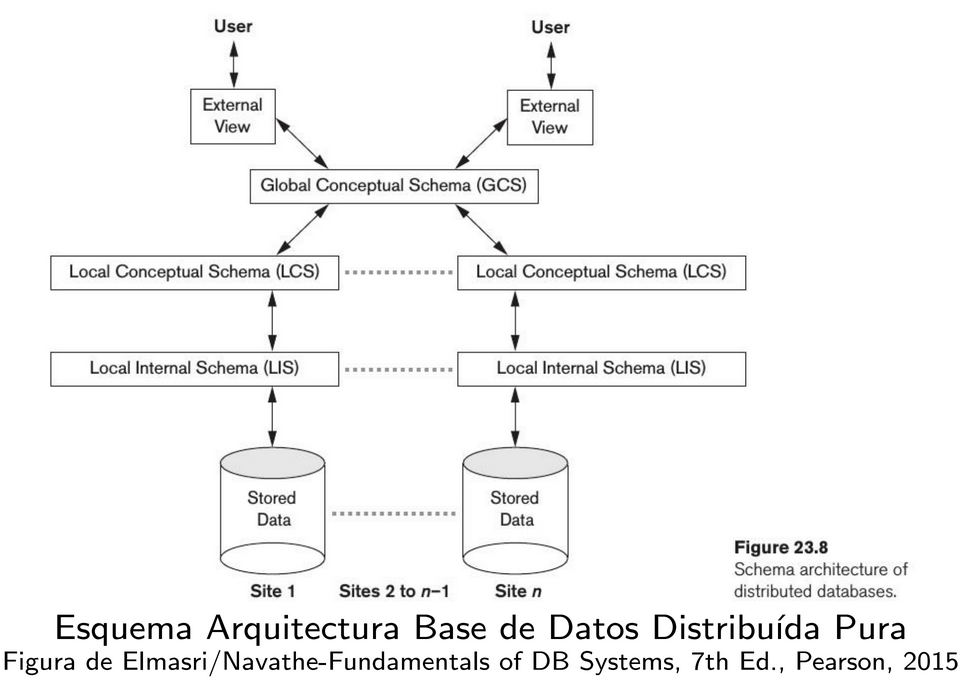
\includegraphics[scale=0.45]{fig/arquitectura-distribuida-pura.png}
    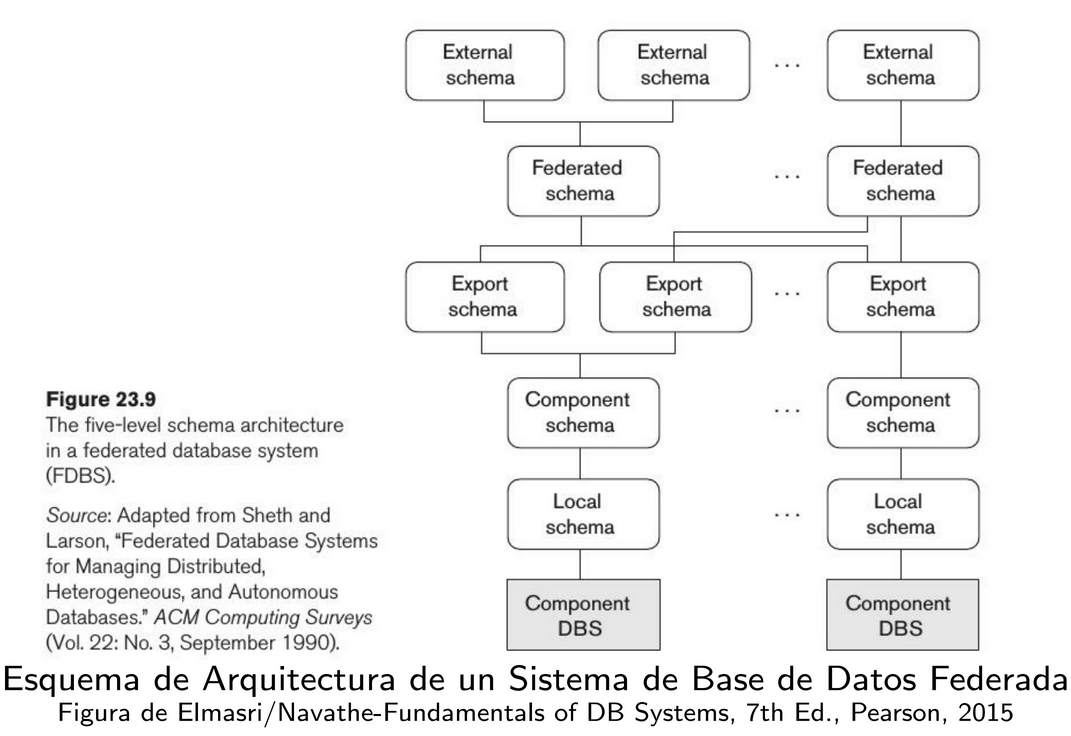
\includegraphics[scale=0.45]{fig/arquitectura-distribuida-federada.png}
\end{figure}



